The refrigeration trailer (hereinafter referred to as reefer trailer) is an insulated trailer designed and built by Schmidt Cargobull with a cooling system developed by Bitzer. It is attached to a truck and has a length of 13.4 meters. The trailer features room for 33 Euro-pallets of cargo and is used to transport various goods that require specific  conditions during transportation, e.g. temperature, humidity and CO2 level. The cooling system used to control the internal temperature in the trailer is powered by an internal battery. This allows the reefer trailer cooling to be powered independently of the truck.

While a reefer trailer usually has its own cooling system installed, the reefer trailer in this project utilizes a custom HVAC system designed by BITZER. This system is built to facilitate testing of advanced control strategies.\\

\subsection{A Textbook Refrigeration System}
A textbook example of a refrigeration system is a single stage refrigeration system as depicted in \cref{fig:HVAC_Diagram_std}.

Components - compressor, valve and heat exchangers

Each step. Explained in relation to p-h diagram


A textbook refridgeration system is comprised of 4 components, as depicted in \cref{fig:HVAC_Diagram_std}. While the refrigerant moves through these components the refridgerant changes temperature, pressure and enthalpy, and goes through phase shifts. These changes are nessesary to ensure that adequately cold liquid refridgerant enters the evaporator to extract heat from the cargo hold. Warm air from the cargo hold is blown over the evaporator pipes, cooling the air before it returns to the cargo hold, allowing for cooling of the cargo in the reefer trailer. 

\begin{figure}[h!]
	\centering
	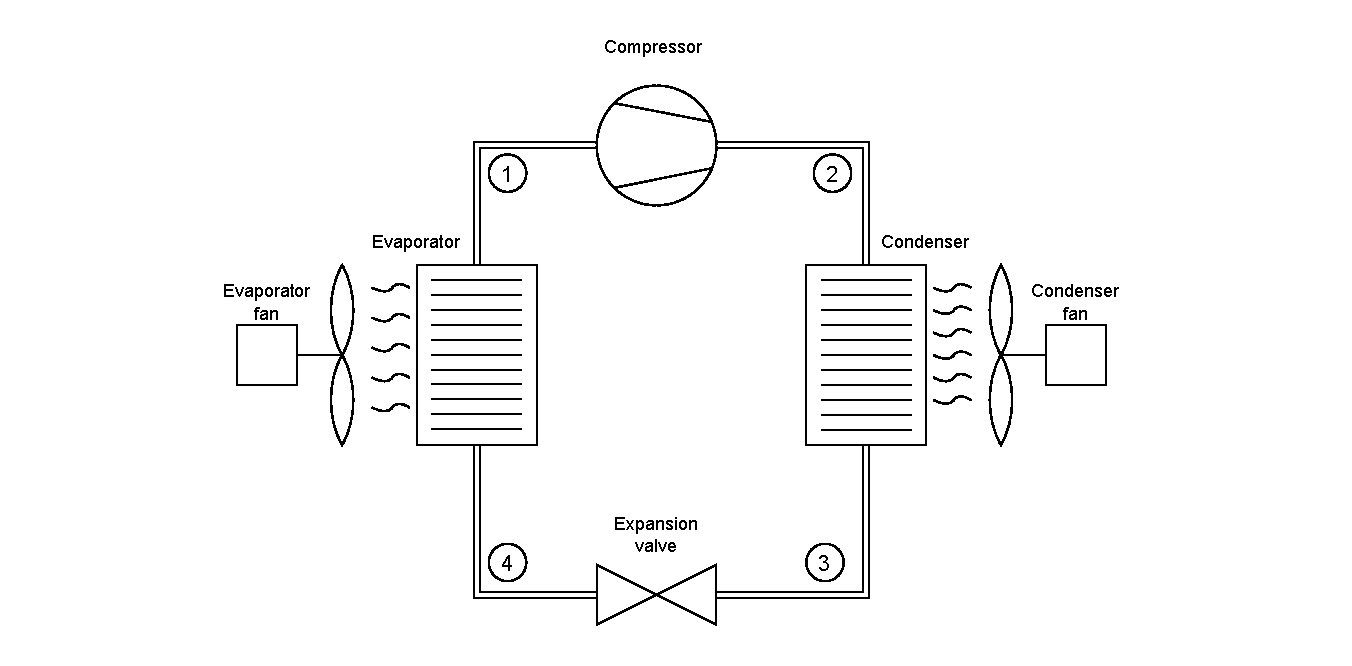
\includegraphics[width=0.85\textwidth]{Graphics/HVAC_Diagram_std.pdf}
	\caption{Illustration of a standard refrigeration cycle}
	\label{fig:HVAC_Diagram_std}
\end{figure}

\begin{figure}
	\centering
	\begin{minipage}{0.45\textwidth}
		\centering
		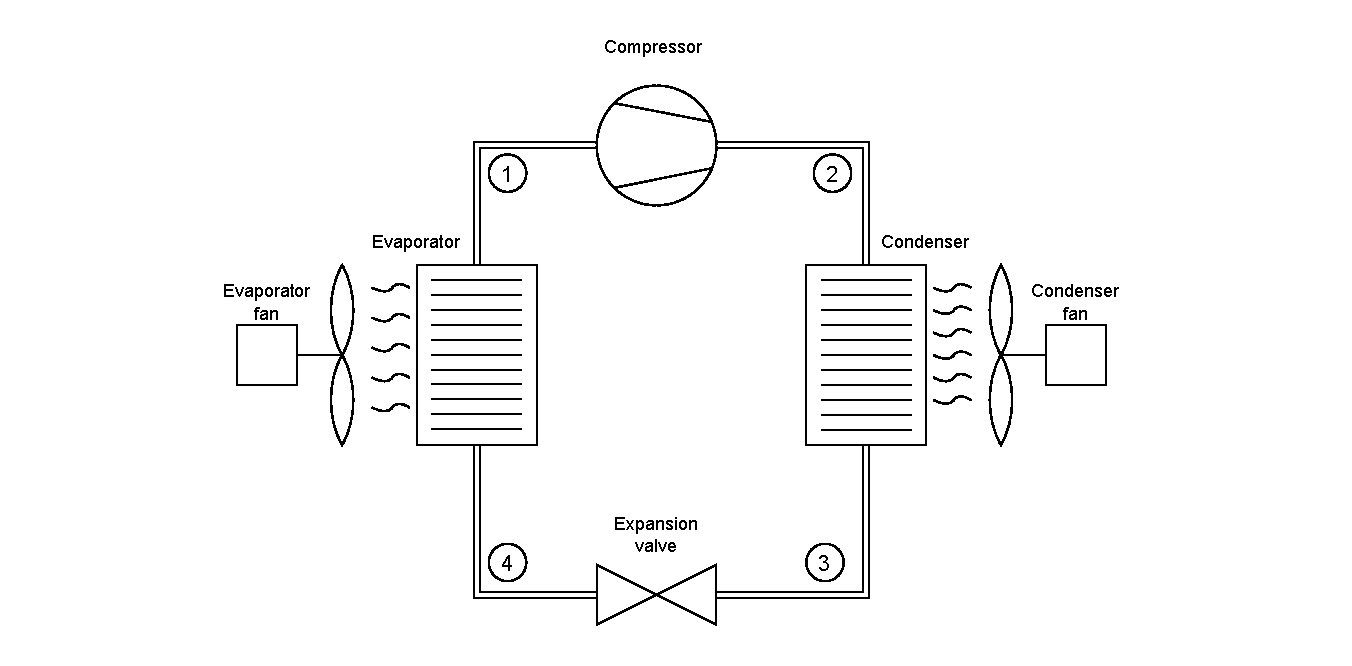
\includegraphics[width=0.9\textwidth]{Graphics/HVAC_Diagram_std.pdf} % first figure itself
		\caption{first figure}
	\end{minipage}\hfill
	\begin{minipage}{0.45\textwidth}
		\centering
		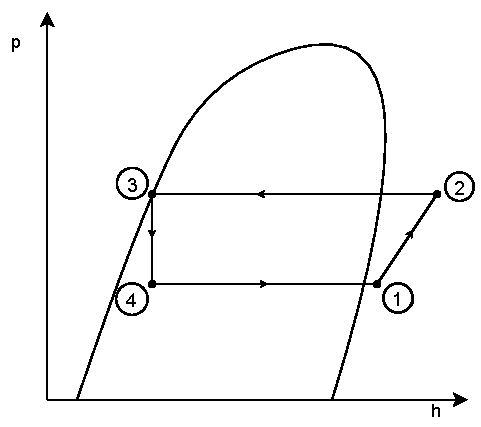
\includegraphics[width=0.9\textwidth]{Graphics/p-h_diagram_std} % second figure itself
		\caption{second figure}
	\end{minipage}
\end{figure}

The pressure and enthalpy of the refridgerant as the four connection points can be plotted in a p-h diagram. \cref{fig:p-h_diagram_std} shows the ideal p-h diagram for the standard refridgeration cycle. The evaporator and condenser are seen to ideally only change the enthalpy of the refridgerant. This is because the ideal behavior is for the refridgerant to go through a phase shift in these components. The expansion valve simply lowers the pressure without changing the enthalpy. This in turn lowers the temperature. The compressor increases the pressure of the refridgerant, while also slightly increasing the enthalpy. This is because ideal compression is an isentropic process, which means the entropy is held constant. Increasing the pressure while keeping entropy constant, requires an increased enthalpy. \\


\begin{figure}[h!]
	\centering
	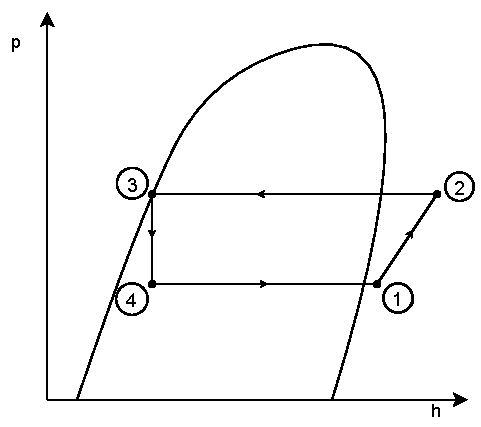
\includegraphics[width=0.55\textwidth]{Graphics/p-h_diagram_std}
	\caption{p-h diagram of the standard refrigeration cycle}
	\label{fig:p-h_diagram_std}
\end{figure}


The refridgeration system implemented in the trailer used in this project contains more components than the standard example. An seen in figure \cref{fig:HVAC_Diagram}, the compressor is comprised of two stages, rather than one. Similarly two valves are being used. They are seperated by a flash tank, that passes flash gas from the condenser throttle valve to the second stage of the compressor. Note, that the subcooling throttle valve is only used for debugging purposes, and is fully open at all times in this project.

\begin{figure}[h!]
	\centering
	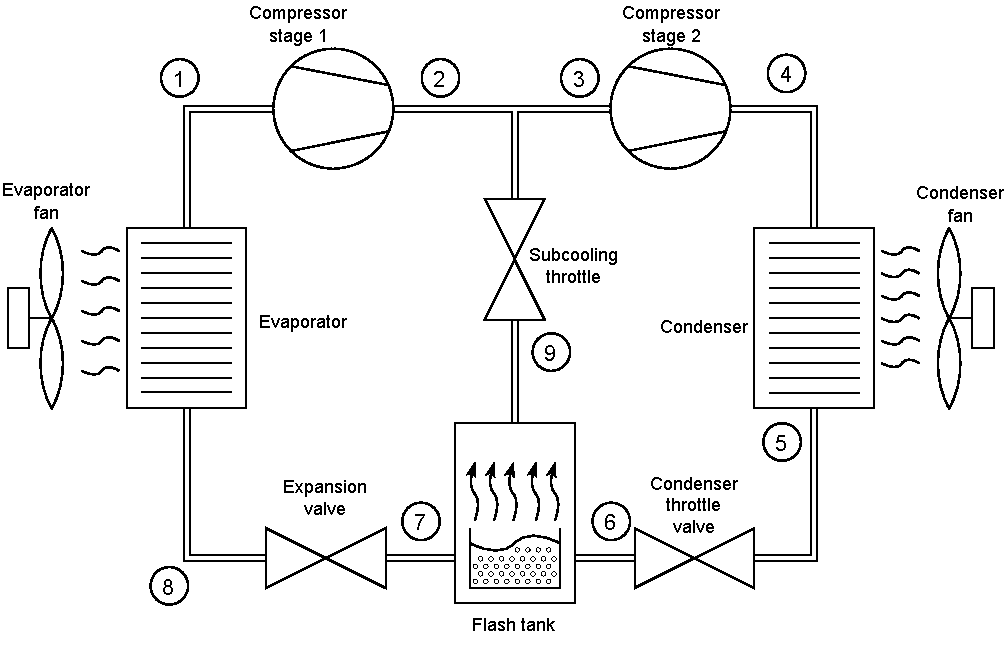
\includegraphics[width=0.85\textwidth]{Graphics/HVAC_Diagram_Fans.pdf}
	\caption{Illustration of refrigeration cycle}
	\label{fig:HVAC_Diagram}
\end{figure}

%It is not accurate but merely depicts the concept of how the enthalpy and pressure changes throughout the cycle.
In \cref{fig:p-h_diagram} an illustrative p-h diagram of this refrigeration cycle can be seen.  The numbers in the figure are also shown in \cref{fig:HVAC_Diagram} for reference. Two cycles can be observed on the diagram. The first is the main cycle which runs along the cycle from point $1 \rightarrow 2\rightarrow 3 \rightarrow 4 \rightarrow 5 \rightarrow 6 \rightarrow 7 \rightarrow 8 \rightarrow 1$ and the second is the cycle running along the cycle from $3 \rightarrow 4 \rightarrow 5 \rightarrow 6 \rightarrow 9 \rightarrow 3$. \\


The purpose of the flash tank is to remove flash gas from the first expansion of the gas in the condenser throttle valve. This reduces the enthalpy of refridgerant continuing to the expansion valve which increases the cooling efficiency of the refrigeration.\\

\begin{figure}[h!]
	\centering
	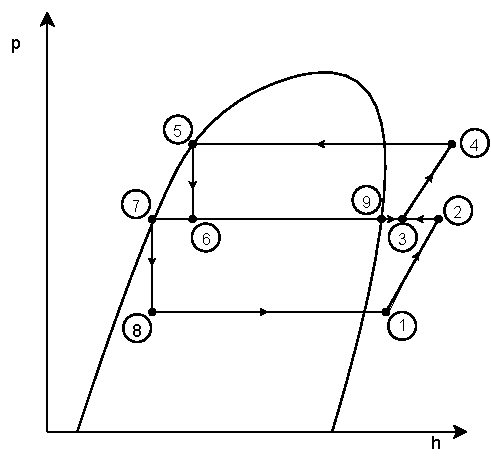
\includegraphics[width=0.55\textwidth]{Graphics/Flash_Tank_P-h_Diagram}
	\caption{p-h diagram of the refrigeration cycle}
	\label{fig:p-h_diagram}
\end{figure}


The system components have variables that can be set to control their behavior. These are the controlled inputs:

\begin{itemize}
	\item The compressor speed $ \omega $
	\item The condenser fan speed $ U_{fan1} $
	\item The evaporator fan speed  $ U_{fan2} $
	\item The condenser throttling valve opening degree $ \Theta_1 $
	\item The expansion valve opening degree $ \Theta_2 $
\end{itemize}

There are several variables such as pressure and temperature throughout the refrigeration cycle, which are measured and hence are outputs of the system. 

The controlled outputs however, are those of interest from a control point of view. These are the outputs that the control strategy seeks to keep at a set point. In this project it will be the trailer box air temperature and the evaporator superheat. Controlling the air temperatur is nessesary to ensure proper storage conditions for the cargo. Regulating the superheat is a more complex objective, as having a large amount of superheat is wasteful and decreases the overall energy efficiency of the trailer. There should however be some amount of superheat, to ensure no liquid refridgerant enters the compressor, since that is destructive to the mechanical system.\\

The aim of the project is to design a Multiple-Inputs-Multiple-Outputs (MIMO) state space controller to keep the temperature inside the container constant despite exogenous inputs (disturbances), specifically the ambient temperature. Furthermore it should do so with the sub-goal of minimizing the energy consumption, primarily by regulating the superheat.\\





\subsection{High-Fidelity model}
When working with a any large scale plant, testing iteratively on the physical system is often impractical. Slow dynamics and inconvienient test procedures make the proces tedious for the user, but there is also the risk of equipment damage. Therefore, it is common practice to develop a high-fidelity model of the system. Testing can be performed efficiently and with no risk on the model. \\

BITZER has created such a Hi-Fi model for the cooling trailer in Simulink. The model has been shown to be highly accurate and can be trusted to mimic the real system behavior in most use-cases. The Hi-Fi model simulates the refridgeration system in \cref{fig:HVAC_Diagram}. The controlled inputs are regulated by a decoupled PID network. The cargo hold air temperature is regulated to -5$^{\circ}$C.\\

The control strategy developed in this project, will first and foremost be tested on the Hi-Fi model. 




\subsection{Problem structure}

The controller will require access to relevant system information. In the context of state space control, this is the values of the system states. The states will be discussed in details later in the report. The states are used for feedback when choosing the proper control signals. Since the states of complex systems are usually not directly measurable, a simple model will be developed for state observation. The model is then to be used for controller design. \\

The control model will be developed by means of first principle modelling. Doing so yields a non-linear model, due to the non-linear physical properties of thermodynamical systems. To apply linear control strategies, the model must be linearised. Optimal control strategies will be implemented on the linear model, as the control objectives can be well formulated as an optimization problem. The optimization problem in this project will be to keep the controlled outputs fixed, while minimizing the energy consumption of the system.\\


		
